\documentclass[conference]{IEEEtran}
\IEEEoverridecommandlockouts
% The preceding line is only needed to identify funding in the first footnote. If that is unneeded, please comment it out.
\usepackage{cite}
\usepackage{amsmath,amssymb,amsfonts}
\usepackage{algorithmic}
\usepackage{graphicx}
\usepackage{textcomp}
\usepackage{xcolor}
\def\BibTeX{{\rm B\kern-.05em{\sc i\kern-.025em b}\kern-.08em
T\kern-.1667em\lower.7ex\hbox{E}\kern-.125emX}}
\begin{document}

    \title{Vehicle Accident Prevention System at Hairpin Turns\\{
    \large Using IR Sensors and Arduino
    }

        }

    \author{\IEEEauthorblockN{Kedar Salunkhe}
    \IEEEauthorblockA{
    Roll no. C54 \\
    PRN no. 2122000465}
    \and
    \IEEEauthorblockN{Sandip Sannake}
    \IEEEauthorblockA{
    Roll no. C59 \\
    PRN no. 2122000621}
    \and
    \IEEEauthorblockN{Abhijit Shende}
    \IEEEauthorblockA{
    Roll no. C63 \\
    PRN no. 2122000659}
    \and
    \IEEEauthorblockN{Tejas Chavan}
    \IEEEauthorblockA{
    Roll no. C70 \\
    PRN no. 2122000357}
    \and
    \IEEEauthorblockN{Digvijay Patil}
    \IEEEauthorblockA{
    Roll no. 71 \\
    PRN no. 2122000814}

    }

    \maketitle

    \begin{abstract}
        In the world, India ranks top in road accidents. Mainly road accidents are caused due to High speed
        or when the driver is not aware of the other vehicles coming opposite to it especially in the deep curves.
        Such types of curves are called as HAIR PIN CURVES. The existing system makes use of convex mirrors
        at the curves so that the driver can easily detect the vehicle coming in the opposite direction. This system
        works well during the day but not effective in night. The proposed system makes use of sensors at hairpin
        curves which work very efficiently during the night time. Placing the sensors at each side of the curves will
        help us to solve the problem. The usage of sensors is that if the vehicle is 10 meters away from the curve the
        sensor sends the signal to the vehicle coming in opposite direction in the form of light. In the same way the
        sensor at the other side of the curve will send signal to the vehicle coming from the opposite direction. In
        this way by using sensors we can avoid a greater number of accidents mainly at the deep curves. Reducing
        the rate of accidents increases the well-being of a person.
    \end{abstract}

    \begin{IEEEkeywords}
        Arduino , Cables , Connector , IR Sensors , Buzzers , Power Supply , PCB Breadboards , Hairpin Bends.
    \end{IEEEkeywords}

    \section{Problem Definition}
    According to million death study (MDS) about 2.3 million people die in India per year. In that 137K is because of road accidents.
    That about 377 peoples per day. In that 3.7\% are because of unexpected obstacles.There are many risky roads and bends in the world
    like mountain roads, narrow curve roads and hair pin bends for ex. Kolli hill roads, Gata Loops,3-Level Zig-zag roads in Sikkim,
    Leh Manali Highway.
    \newline
         Hairpin turns are often built when a route climbs up or down a steep slope, so that it can travel mostly
    across the slope with only moderate steepness and are often arrayed in a zigzag pattern. Highways with
    repeating hairpin turns allow easier, safer ascents and descents of mountainous terrain than a direct, steep
    climb and descent, at the price of greater distances of travel and usually lower speed limits, due to the
    sharpness of the turn. Highways of this style are also generally less costly to build and maintain than
    highways with tunnels. Hairpin curves are used when the terrain is very steep. Roadways will have a
    maximum grade that a vehicle or truck can traverse. The zigzag component of the picture above minimizes
    the grade, or steepness of the roadway. If you have ever ridden a bike up a steep hill, you might have found
    yourself zigzagging back and forth across the roadway to get up the hill. The same principle applies here.
    When designing a roadway, there are guidelines as to the length of the radius of curve based primarily on
    the design speed. The faster the designs speed, the longer the radius of the curve. Truck traffic is a major
    factor in the design criteria for the minimum radius of curvature. Turning templates are used to determine if
    a truck can make the turn without too much of tracking. A bend in a road with a very acute inner angle,
    making it necessary for an oncoming vehicle to turn almost 180° to continue on the road. Such turns in
    ramps and trails may be called switchbacks in American English. While driving on roads at hairpin section,
    many drivers face accident which results them into serious injuries or even death. The main reason behind
    this accident is curves and bends of roads while turning in Ghats. It becomes difficult to see vehicles coming
    from other lane and turning drivers usually have to assume a way for turning at such critical section this
    creates a great risk of life other reason for accident in hairpin section is that only one vehicle can turn at
    turnings at a time. If two vehicles come face to face while turning, it creates a chance of accidents and it
    becomes difficult to handle. At night, due to no streetlights it becomes a difficult task of driving on hairpin
    bends and especially while turning. It becomes more difficult at night to make a turn as vehicle coming from
    another side of road is not visible due to darkness.
    \begin{figure}[htbp]
        \centerline{\includegraphics[scale=0.5]{arduino-connector}}
        \caption{Connector cable}
        \label{fig}
    \end{figure}

    \section{Literature Review}

    \subsection{“Sensor Based Accident Prevention System” Author: Aravinda B, Chaithra Lakshmi C, Deeksha, Ashutha K[1]}

    This paper is introducing sensor based accident prevention system:- That is we are keeping ultrasonic sensor in one side of the road
    before the curve and keeping a LED light after the curve. Ultrasonic sensor which is also called as obstacle sensor sends signal as
    pulse from trigger. If vehicle is present signal will hit the vehicle and it is received by the sensor. At that time light will glow at the
    other side of the curve. In the absence of the vehicle the light will not glow because the signal will not be received by the sensor. As
    the signal senses the vehicle light will glow that is indication to driver that some vehicle is arriving from the front side. The driver
    get noticed the signal and slow down or stop the vehicle if necessary. This type of sensor based light system can be applicable when
    the driver unable to see the vehicle coming from other end of the road. Using this idea we can make all the mountain roads and
    curve roads safer from accidents and can save thousands of lives a year. The aim of this paper is to decrease the number of accidents
    in curve roads. This is done by alerting the driver by means of LED light which glows when vehicle comes from the other side of
    the curve. The vehicle is detected by the help of Ultrasonic sensor which is interfaced to the micro controller Arduino UNO. By this
    we can save thousands of lives in the curve roads.[1]
    
    \subsection{“Diminishing Road Accidents On Sharp Curves Using Arduino”. Ranga Sreedhar Galla [2]}
    Has studied the main purpose of this paper is to reduce accidents on hilly and slippery roads. In curve roads the other road end of
    vehicle cannot seen by driver. At night many time accidents may happens by huge intensity of head light from opposite side of
    vehicles. Also, the light intensity problem occurs both curved roads and mountain roads at night because of these type of problem
    Thousands of people lose their lives. The solution for this problem is alerting the driver about the vehicle coming from opposite
    side. This is done by keeping an ultrasonic sensor in one side of the road before the curve and keeping a LED light after the curve,
    so that if vehicle comes from one end of the curve sensor senses and LED light glows at the opposite side.[2]
    
    \subsection{“Smart Road Safety and Vehicle Accident Prevention System for Mountain Roads” Kartik Venkata Mutya, Sandeep Rudra[3]}
    Has studied the road traffic accidents are being recognized as a major public health problem in number of countries with alarmingly
    increasing fatalities in developing countries. Careless and rash driving as a result of excessive waiting and blind corners is attributed
    as one of the most important factor for all road accidents. An estimated 1.2 million people lose their lives in road traffic crashes
    every year, and another 20 to 50 million are injured. A docile, economical mechanism to prevent these road accidents is the need of
    the hour. It is hoped that the mechanism presented in this article would help in alleviating this concern especially in correspondence
    with large vehicle accidents on highways by being easily implemented in low income countries and this mechanism can save
    thousands of life.[3]
    
    \subsection{R. Saranya, R. Arun Kumar [4]}
    This paper conclude that, Accidents may takes place in various factors drunk and driving, Texting while driving, Speeding,
    Distractions, Sleeping while driving. Among Drowsiness is reason for most of the accidents. While driving at the speed of
    100km/hr. driver falls sleepy within 4 seconds the buzzer will enables.[4]
    
    \subsection{“Implementation of Vehicle Mishap Averting System Using Arduino Microcontroller”,R.S Rakul[5]}
    The Unit has been designed to prevent an accident by collision. The ‘heart' of the Unit is
    Arduino microcontroller which performs all the vital tasks of the system. And it will be discussed in the
    following subsequent sections. This system will receive information from the Ultrasonic transceiver, and
    accordingly transmit the data via the Wi-Fi router to the controller. Through the buzzer indication, light
    emitting display, and liquid crystal display, the vehicle information will be shown to the vehicle users. The
    primary purpose of the system is to prevent collision between two or more vehicles when they take a turn on
    U-bends.[5]

    \section{Synopsis of Literature Review}
    The purpose of these papers is to reduce the number of
    accidents in curve roads. This is done by warning the driver
    by means of LED light which glows when vehicle comes from
    the other side of the curve. The vehicle is detected by the
    help of IR Transmitter and Receiver sensor which is
    interfaced to the microcontroller arduino Uno. In this we can
    save thousands of lives in the curve roads on the ghat
    section.

    \section{Project Plan}

    \subsection{Setup}
    \subsubsection{Setting up the Arduino}
    We used the Arduino IDE to write and upload the code via the cable
    \begin{figure}[htbp]
        \centerline{\includegraphics[scale=0.5]{arduino-connector}}
        \caption{Connector cable}
        \label{fig}
    \end{figure}


    \begin{verbatim}
int irSensor = 12;
int buzzer = 7;
void setup()
{
  Serial.begin(9600);
  pinMode(irSensor, INPUT);
  pinMode(buzzer, OUTPUT);
}
void loop()
{
  int value = digitalRead(irSensor);
  Serial.println("");
  Serial.print("Sensor Value = ");
  Serial.print(value);

  if(value == 0)
  {
    digitalWrite(buzzer, HIGH);
  }
  else
  {
    digitalWrite(buzzer, LOW);
  }
  delay(50);
}
    \end{verbatim}
    \subsubsection{Connecting sensors}
    We use jumper wires to connect the arduino to sensor and buzzer
    \begin{figure}[htbp]
        \centerline{\includegraphics[scale=0.15]{connection}}
        \caption{Jumer wire connection}
        \label{fig}
    \end{figure}

    \subsubsection{Final model}

    This is the final connection. The LED is connected after the model is completed.
    A 9V battery is used as power source for the arduino.
    \begin{figure}[htbp]
        \centerline{\includegraphics[scale=0.15]{final-connection}}
        \caption{Final connection}
        \label{fig}
    \end{figure}
    \section{Sketch}

    \subsection{Block diagram}
    \begin{figure}[htbp]
        \centerline{\includegraphics[scale=0.3]{block-diagram}}
        \caption{Block Diagram}
        \label{fig}
    \end{figure}

    \subsection{Schematic Diagram}
    \begin{figure}[htbp]
        \centerline{\includegraphics[scale=0.75]{schematic-diagram}}
        \caption{Schematic Diagram}
        \label{fig}
    \end{figure}
    \section{Components Required}


    \subsection{ARDUINO UNO}\label{AA}
    The Arduino Uno is a microcontroller board which is open
    source used to insert the code as input using USB and can get
    the excepted output.This platform consists of physical
    programmable path board or IDE(Integrated Development
    Environment) that runs on computer, used to mark and
    upload computer code to the physical board. The
    ATmega328 on the board comes preprogrammed with a
    boot loader that allows uploading new code to it without the
    use of an outside hardware programmer. Arduino board
    design uses a mixture of microprocessors and controllers.
    The
    boards
    are
    set
    with
    digital
    and
    analog input/output (I/O) pins that may be interfaced to a
    choice of development boards or breadboards (For
    prototyping) and other circuits. The microcontrollers can be
    programmed using C and C++ programming languages [3].

    \begin{figure}[htbp]
        \centerline{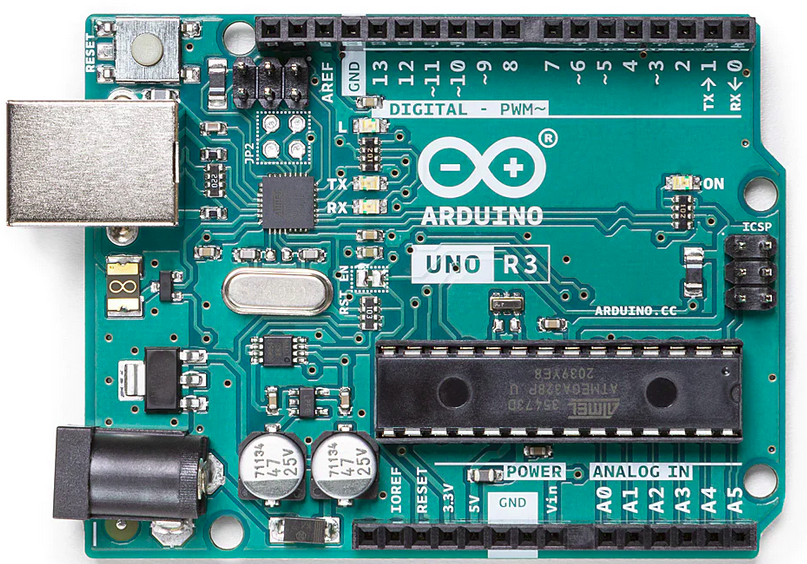
\includegraphics[scale=0.30]{fig3.png}}
        \caption{Arduino UNO top view}
        \label{fig}
    \end{figure}

    \subsection{IR SENSOR}
    Infrared sensors are being used as proximity sensors and
    they can be passive or active. Passive infrared sensors are
    basically Infrared detectors. These sensors do not use any
    infrared source and detects energy emitted by obstacles in
    the field of view. The active infrared sensors consist of two
    elements which are infrared source and infrared detector.
    Infrared source includes an infrared laser diode. Infrared
    detectors include photodiodes or phototransistors. The
    energy emitted by the infrared source is reflected by a
    purpose and falls on the infrared detector. An IR sensor
    consists of an IR LED then an IR Photodiode; mutually they
    are called as Photo – Coupler or Opto – Coupler. When the IR
    transmitter emits radiation, it reaches the thing and some of
    the radiation reflects reverse to the IR receiver. Based on the
    force of the reception by the IR receiver, the output of the
    sensor is defined [4].

    \begin{figure}[htbp]
        \centerline{\includegraphics[scale=0.25]{ir-sensor}}
        \caption{IR Sensor}
        \label{fig}
    \end{figure}

    \subsection{BUZZER}
    An audio signaling device like a beeper or buzzer may be electromechanical or piezoelectric or mechanical type. The main function of this is to convert the signal from audio to sound. Generally, it is powered through DC voltage and used in timers, alarm devices, printers, alarms, computers, etc. Based on the various designs, it can generate different sounds like alarm, music, bell & siren
    \begin{figure}[htbp]
        \centerline{\includegraphics[scale=0.25]{buzzer}}
        \caption{Buzzer}
        \label{fig}
    \end{figure}


    \subsection{LED LIGHTS}
    \paragraphA Light Emitting Diode (LED) is an electronic device of a
    semi-conductor source that emits light when an electrical
    current is passed through it. The early LEDs are to produce
    only red light, but the current LEDs can produce several
    different colors, including red, green, and blue (RGB) light.
    The recent advances in LED technology have made it
    probable for LEDs to produce white light as well. LEDs are
    generally used for indicator lights (such as power on/off
    lights) on electronic devices. They also have few other
    applications, with electronic signs, clock displays, and
    flashlights. You can typically identify LEDs by a series of small lights that make up a bigger display. The capable
    nature of LEDs allows them to produce brighter light than
    other types of bulbs while using less energy [5].

    \begin{figure}[htbp]
        \centerline{\includegraphics[scale=0.25]{led.jpg}}
        \caption{LED}
        \label{fig}
    \end{figure}

    \begin{figure}[htbp]
        \centerline{\includegraphics[scale=0.15]{jumper-wires}}
        \caption{Jumper Wires}
        \label{fig}
    \end{figure}


    \subsection{OTHER ITEMS}
    \itemize
    \item Resistors
    \item Transistors
    \item Diodes
    \item Push buttons
    \item IC
    \item Capacitors
    \item Cables and Connectors
    \item PCB and Breadboard
    \enditemize


    \section{Working Mechanism}
    It uses an IR sensor, which is
    placed on one side of the hairpin bend. This IR sensors
    are senses by the side of the downhill section of the road.
    The sensors is connected to
    ATmega328P microcontroller through wires. Based on the
    output of sensors, position of vehicles on other side of the
    bend is detected which is provided as an input to the
    microcontroller. The microcontroller which works on a
    power supply of 9V runs a Priority algorithm which triggers
    the warning LEDs to glow and thereby intelligently
    controlling the movement of vehicles at the bend. Warning
    LEDs are placed at the side of the uphill section of the
    hairpin bend

    \section{Conclusion}
    The experiment are started with sensor, it senses the vehicle
    with the help of IR Sensor. In this project we are alert the
    driver by blinking. The clash avoidance at hairpin bend is
    able to transmit data which is sensed from other side of the
    road. The system is completely integrated and can give alert
    to the driver by using LED. This system helps to detect the
    vehicles by Using their IR Sensor. This system provides the
    information about the vehicles coming from the opposite side of the vehicles in the Ghats section. This system is useful
    when the driver can't see the vehicle in the opposite side of
    the vehicle because of long curve roads in the Ghats section.
    Thus the system offers the safety and security to the driver.
    \section{Future Scope}
    \itemize
    \item[1] Arrangements to protect the sensor from being damaged in critical places.
    \item[2] Decrease the size of unit so that it occupies small place and easily kept in narrow roads.
    \item[3] Implementing the system to detect number of vehicles and velocity of vehicle and try to specticate the natural calamities if
    happen alert may rise on buzzer for no further accidents.
    \section*{Acknowledgment}

    Thanks to Mrs. Ashwini Choughule Ma'am for guiding us through the project


    \begin{thebibliography}{00}
        \bibitem{b1} S. Kaplan and C. G. Prato, “Risk factors associated with bus accident severity in the United States: a generalized ordered logit model,” Journal of Safety
        Research, vol. 43, no. 3, pp. 171–180, 2012.
        \bibitem{b2} RANGA SREEDHAR GALLA Diminishing Road Accidents On Sharp Curves Using Arduino Volume 1 Issue 5, November 2017.
        \bibitem{b3} Jessen Joseph Leo., R. Monisha.,et.al. : Vehicle movement control and accident avoidance in hilly track, IEEE Int. Conf. on Electronics and Communication
        Systems (ICECS).pp. 1-5(2014).
        \bibitem{b4} DEEKSHA ASHUTHA K. ARAVINDA B, CHAITHRA LAKSHMI C. Sensor based accident prevention system. International Journal of Computer
        Applications, pages 36–39, 2012.
        \bibitem{b5} R.S. Rakul, S. Ravia and K.N. Thirukkuralkani proposed a paper on “Implementation Of
        Mishap Averting System Using Arduino Microcontroller”.
        \end{thebibliography}

\end{document}

